% \documentclass{beamer}
\documentclass[xcolor=dvipsnames]{beamer}
\usefonttheme{serif}
%% \usecolortheme[named=Blue]{structure}
\setbeamersize{text margin left=30mm, text margin right=30mm}
\useoutertheme{infolines}
%% \usetheme[height=7mm]{Rochester}
\usetheme{Pittsburgh}
\setbeamertemplate{items}[ball]
\setbeamertemplate{blocks}[rounded][shadow=true]
\setbeamertemplate{navigation symbols}{}

\usepackage[utf8x]{inputenc}
%% \usepackage{default}
\usepackage[english]{babel}
\usepackage{geometry}
%% \usepackage{fullpage}
\usepackage{amsmath, amsthm, amssymb}
\usepackage{listings}
\usepackage{pxfonts}
\usepackage{caption}

%% \usepackage{color}
%% \usepackage{graphicx}
%% \usepackage{natbib}
%% \usepackage{array}
%% \usepackage{booktabs}
%% \usepackage{tabu}
%% \usepackage[utf8]{inputenc}
%% \usepackage{fancyhdr}
%% \usepackage{float}
%% \usepackage{subfigure}
%% \usepackage{titlesec}

\setbeamertemplate{headline}{}
\setbeamertemplate{footline}[frame number]{}
\setbeamertemplate{navigation symbols}{}
\setbeamertemplate{footline}{}
\setbeamertemplate{footline}[frame number]

\setbeamertemplate{itemize items}{$-$}

\def\CCT{{C\nolinebreak[4]\hspace{-.05em}\raisebox{.4ex}{\tiny\bf ++}}}
\def\CC{{C\nolinebreak[4]\hspace{-.05em}\raisebox{.4ex}{\small\bf ++}}}


\definecolor{lstgray}{gray}{0.93}
\definecolor{strgray}{gray}{0.4}

\lstset{ %
  escapechar=@,
  language=C++,
  basicstyle=\footnotesize\ttfamily,
  %% basicstyle=\ttfamily,
  %% keywordstyle=\color{blue}\ttfamily,
  keywordstyle=\bfseries,
  stringstyle=\color{strgray}\ttfamily,
  commentstyle=\color{OliveGreen}\ttfamily,
  %% morecomment=[l][\color{red}]{\#},
  morecomment=[l][\color{blue}]{\#},
  backgroundcolor=\color{lstgray},
  %% keywordstyle=\color{red},
  frame=f,
  frameround=ffff,
  tabsize=2,
  breaklines=true,
  breakatwhitespace=false,
  showspaces=false,
  showstringspaces=false,
  xleftmargin=5pt,
  xrightmargin=5pt,
  morekeywords={in,out,ref,auto,inout,import,ushort,scope,exit,mixin,decltype,varid,sizeof,constexpr}
}

\def\redcolor{\color{red}}
\def\bluecolor{\color{blue}}
\def\blackcolor{\color{black}}
\def\graycolor{\color{gray}}
\def\greencolor{\color{OliveGreen}}


\def\sectionname{\translate{Section}}
\def\insertsectionnumber{\arabic{section}}
\setbeamertemplate{section page}
{
  \begin{centering}
    \begin{beamercolorbox}[sep=4pt,center]{part title}
      \usebeamerfont{section title}\insertsection\par
    \end{beamercolorbox}
  \end{centering}
}
\def\sectionpage{\usebeamertemplate*{section page}}


\AtBeginSection{\frame{\sectionpage}}


\title{What is Marriage?}
\subtitle{`Twelve books' series}
\author{Dominic Jones}
\date{\small{October 2018}}
\institute{\small{\texttt{netherhallhouse.org.uk/books}}}


\begin{document}
\begin{frame}[plain]
  \titlepage
\end{frame}


\begin{frame}{}
  %% \centering
  \begin{quote}
    ``Reason is not just a debater's tool for idly refracting arguments into premises, but a lens for bringing into focus the features of human flurishing''
  \end{quote}

  ~

  \hspace*{8cm}{What is Marriage?}
  \hspace*{3.8cm}{\small{Harvard Journal of Law and Public Policy, 2012}}
\end{frame}


\begin{frame}[plain]
  \begin{columns}[T] % align columns
    %% \begin{column}{0.3\textwidth}
    %% \end{column}%
    %% \hfill%
    \begin{column}{0.9\textwidth}
      \begin{figure}[H]
        \centering
        \includegraphics[width=0.99\textwidth]{reading-group}
      \end{figure}
    \end{column}%
  \end{columns}
\end{frame}


\begin{frame}[plain]
  \begin{columns}[T] % align columns
    %% \begin{column}{0.3\textwidth}
    %% \end{column}%
    %% \hfill%
    \begin{column}{0.99\textwidth}
      \begin{figure}[H]
        \centering
        \includegraphics[width=0.99\textwidth]{marriage}
      \end{figure}
    \end{column}%
  \end{columns}
\end{frame}


%% \begin{frame}[plain]
%%   \begin{columns}[T] % align columns
%%     %% \begin{column}{0.3\textwidth}
%%     %% \end{column}%
%%     %% \hfill%
%%     \begin{column}{0.48\textwidth}
%%       \begin{figure}[H]
%%         \centering
%%         \includegraphics[width=0.99\textwidth]{book}
%%       \end{figure}
%%     \end{column}%
%%   \end{columns}
%% \end{frame}


\section{Two views}


\begin{frame}{The conjugal view}
\begin{quote}
A union between a man and woman, a permanent and exclusive commitment of the type that is inherently fulfilled by bearing and rearing children together
\end{quote}
%% \hspace*{10cm}{p???}
\end{frame}


\begin{frame}[plain]
  \begin{columns}[T] % align columns
    %% \begin{column}{0.3\textwidth}
    %% \end{column}%
    %% \hfill%
    \begin{column}{0.9\textwidth}
      \begin{figure}[H]
        \centering
        \includegraphics[width=0.99\textwidth]{conjugal}
      \end{figure}
    \end{column}%
  \end{columns}
\end{frame}


\begin{frame}{The consentualist view}
\begin{quote}
A union of two people who commit themselves to romantically loving and caring for each other and to sharing the burdens and benefits of domestic life
\end{quote}
%% \hspace*{10cm}{p???}
\end{frame}


\begin{frame}[plain]
  \begin{columns}[T] % align columns
    %% \begin{column}{0.3\textwidth}
    %% \end{column}%
    %% \hfill%
    \begin{column}{0.9\textwidth}
      \begin{figure}[H]
        \centering
        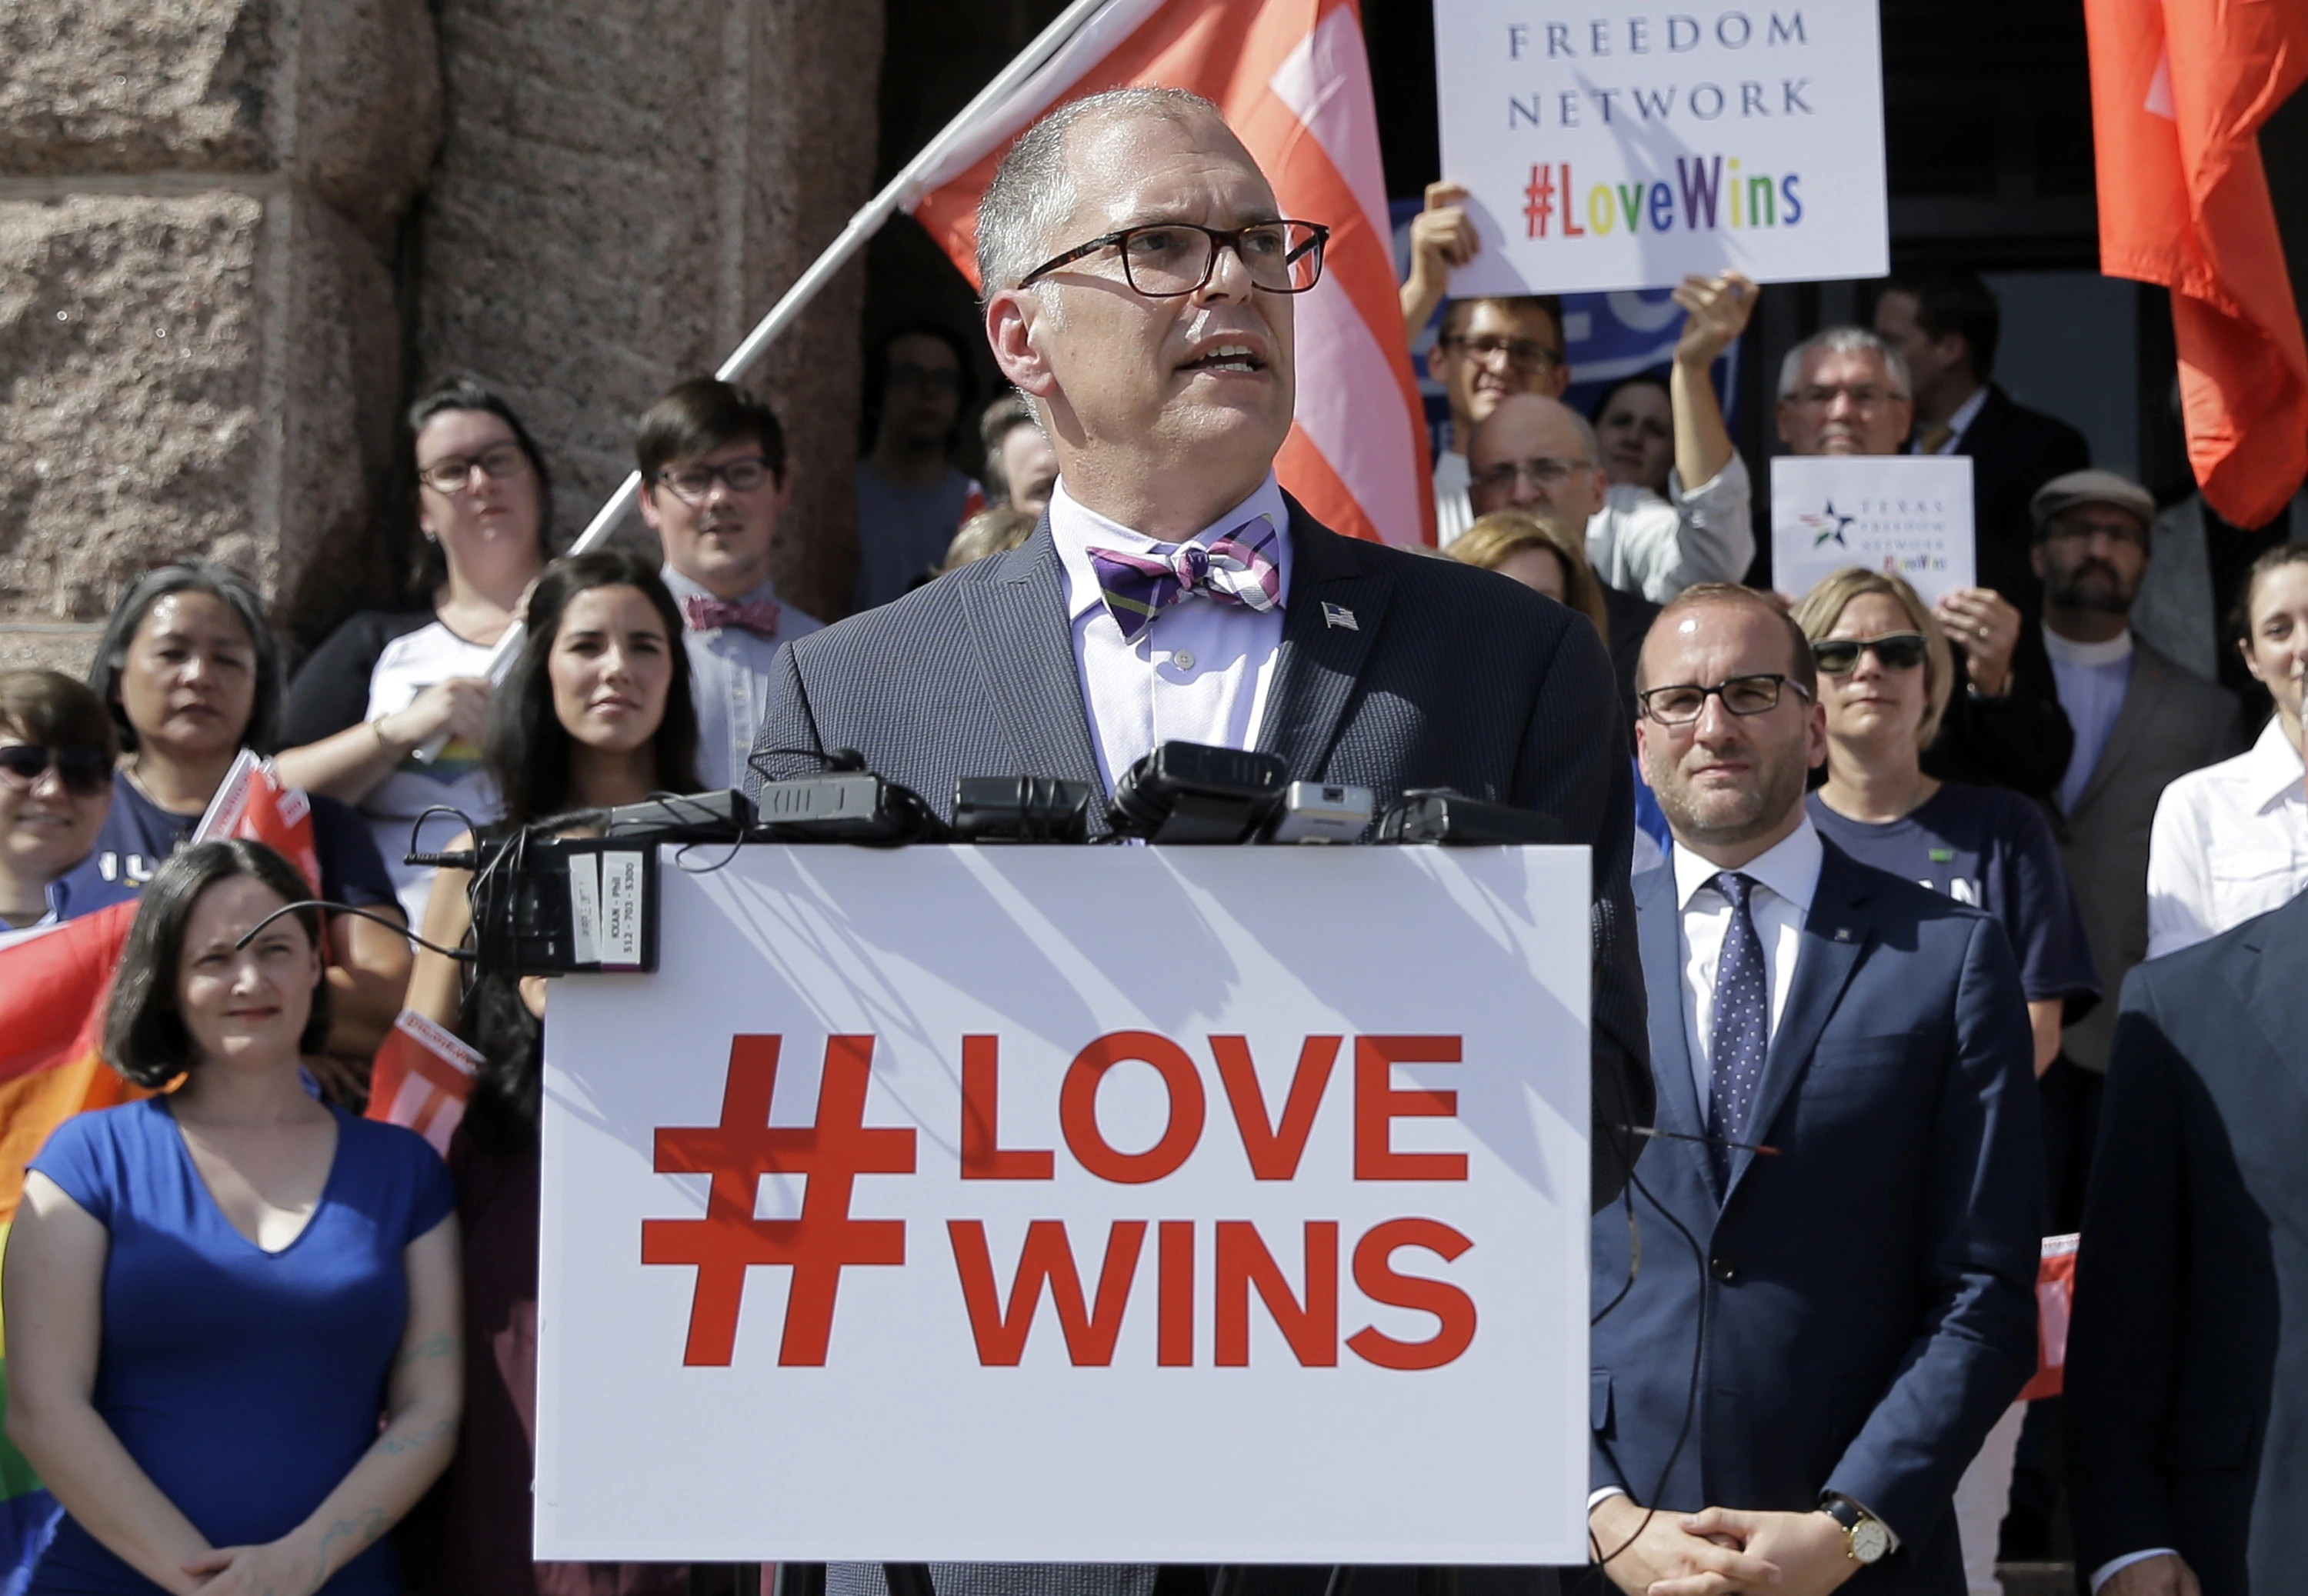
\includegraphics[width=0.99\textwidth]{consentual}
      \end{figure}
    \end{column}%
  \end{columns}
\end{frame}


\section{Seeking legal recognition}


\begin{frame}{This relationship is special because...}
\textbf{We have an emotional loving bond}\newline
But so do parents and children, friends, relatives \vspace{10mm}

\textbf{We may engage in some form of genital activity}\newline
But what act is consummative, if any, and why? \vspace{10mm}

\textbf{We are a couple}\newline
But what is particular to couples so as to exclude three or more? \vspace{10mm}
\end{frame}


\begin{frame}{Enshrining in law}
  \textbf{Is there a real distinction to be made?}\newline
\begin{itemize}
\item Entering, honouring, and terminating a contract
\item Sufficiently well defined
\item Of concern to the common good of society
\item In need of legal protection
\item Capable of bearing responsibility
\item Vunerable dependents
\end{itemize}

~

Ordinary friendship does not affect the political common good in structured ways that justify or warrant legal protection
\end{frame}


\begin{frame}[plain]
  \begin{columns}[T] % align columns
    %% \begin{column}{0.3\textwidth}
    %% \end{column}%
    %% \hfill%
    \begin{column}{0.9\textwidth}
      \begin{figure}[H]
        \centering
        \includegraphics[width=0.99\textwidth]{prenup}
      \end{figure}
    \end{column}%
  \end{columns}
\end{frame}


\section{State of affairs (UK law)}


\begin{frame}[plain]
  \begin{columns}[T] % align columns
    %% \begin{column}{0.3\textwidth}
    %% \end{column}%
    %% \hfill%
    \begin{column}{0.7\textwidth}
      \begin{figure}[H]
        \centering
        \includegraphics[width=0.99\textwidth]{marriage-uk}
      \end{figure}
    \end{column}%
  \end{columns}
\end{frame}


\begin{frame}[plain]
  \begin{columns}[T] % align columns
    %% \begin{column}{0.3\textwidth}
    %% \end{column}%
    %% \hfill%
    \begin{column}{0.7\textwidth}
      \begin{figure}[H]
        \centering
        \includegraphics[width=0.99\textwidth]{annul-uk}
      \end{figure}
    \end{column}%
  \end{columns}
\end{frame}


\section{Organic bodily union}


\begin{frame}{Faculties and coordination}
\textbf{Only one faculty in need of complementarily}\newline
All faculties, except the reproductive, are wholly individual. The reproductive faculties need the two sexes to unite biologically to form a coordinated unity \vspace{10mm}

\textbf{Connection between marriage and children}\newline
The generative act is fulfilled by children, thus is the consummative act \vspace{10mm}

\textbf{Participation is sufficient}\newline
The lack of fulfilment of the act does not nullify the consummation \vspace{10mm}
\end{frame}


\section{Until the love runs out}


\begin{frame}{Permanence and exclusivity}
\textbf{Substantial unity}\newline
Like the union of organs forming a healthy whole person, the stable biological union of man and woman points toward an enduring bond for the life of the parts \vspace{10mm}

\textbf{Concrete focus}\newline
The inherent orientation of conjugal union to children deepens and extends whatever reasons spouses may have to stay together \vspace{10mm}

\textbf{End in itself}\newline
Not a mere means, even to the great good of procreation; it is worthwhile for its own sake \vspace{10mm}
\end{frame}


\section{Undermining friendship}


\begin{frame}[plain]
  \begin{columns}[T] % align columns
    %% \begin{column}{0.3\textwidth}
    %% \end{column}%
    %% \hfill%
    \begin{column}{0.9\textwidth}
      \begin{figure}[H]
        \centering
        \includegraphics[width=0.99\textwidth]{four-loves}
      \end{figure}
    \end{column}%
  \end{columns}
\end{frame}


\begin{frame}{Hidden assumptions}
\begin{itemize}
\item ``Fulfilment is impossible without regular outlets for sexual release''\vspace{5mm}
\item ``Meaningful intimacy is impossible without sex''\vspace{5mm}
\item ``Fulfiling relationships are impossible without legal recognition''\vspace{5mm}
\item ``Homosexual orientation is a basic human identity, such that any state that does not actively accommodate it necessarily harms or disregards a  class of people''\vspace{5mm}
\end{itemize}
\end{frame}


\section{Reading ends in nature}


\begin{frame}{A thought experiment}
\textbf{}\newline
Suppose reproduction was asexual and the off-spring self sufficient.

~

Would any culture have developed an institution anything like what we know as marriage? \vspace{10mm}
\end{frame}


\begin{frame}[plain]
  \begin{columns}[T] % align columns
    %% \begin{column}{0.3\textwidth}
    %% \end{column}%
    %% \hfill%
    \begin{column}{0.99\textwidth}
      \begin{figure}[H]
        \centering
        \includegraphics[width=0.99\textwidth]{cs-lewis}
      \end{figure}
    \end{column}%
  \end{columns}
\end{frame}


\end{document}
